\begin{figure}
    \centering
    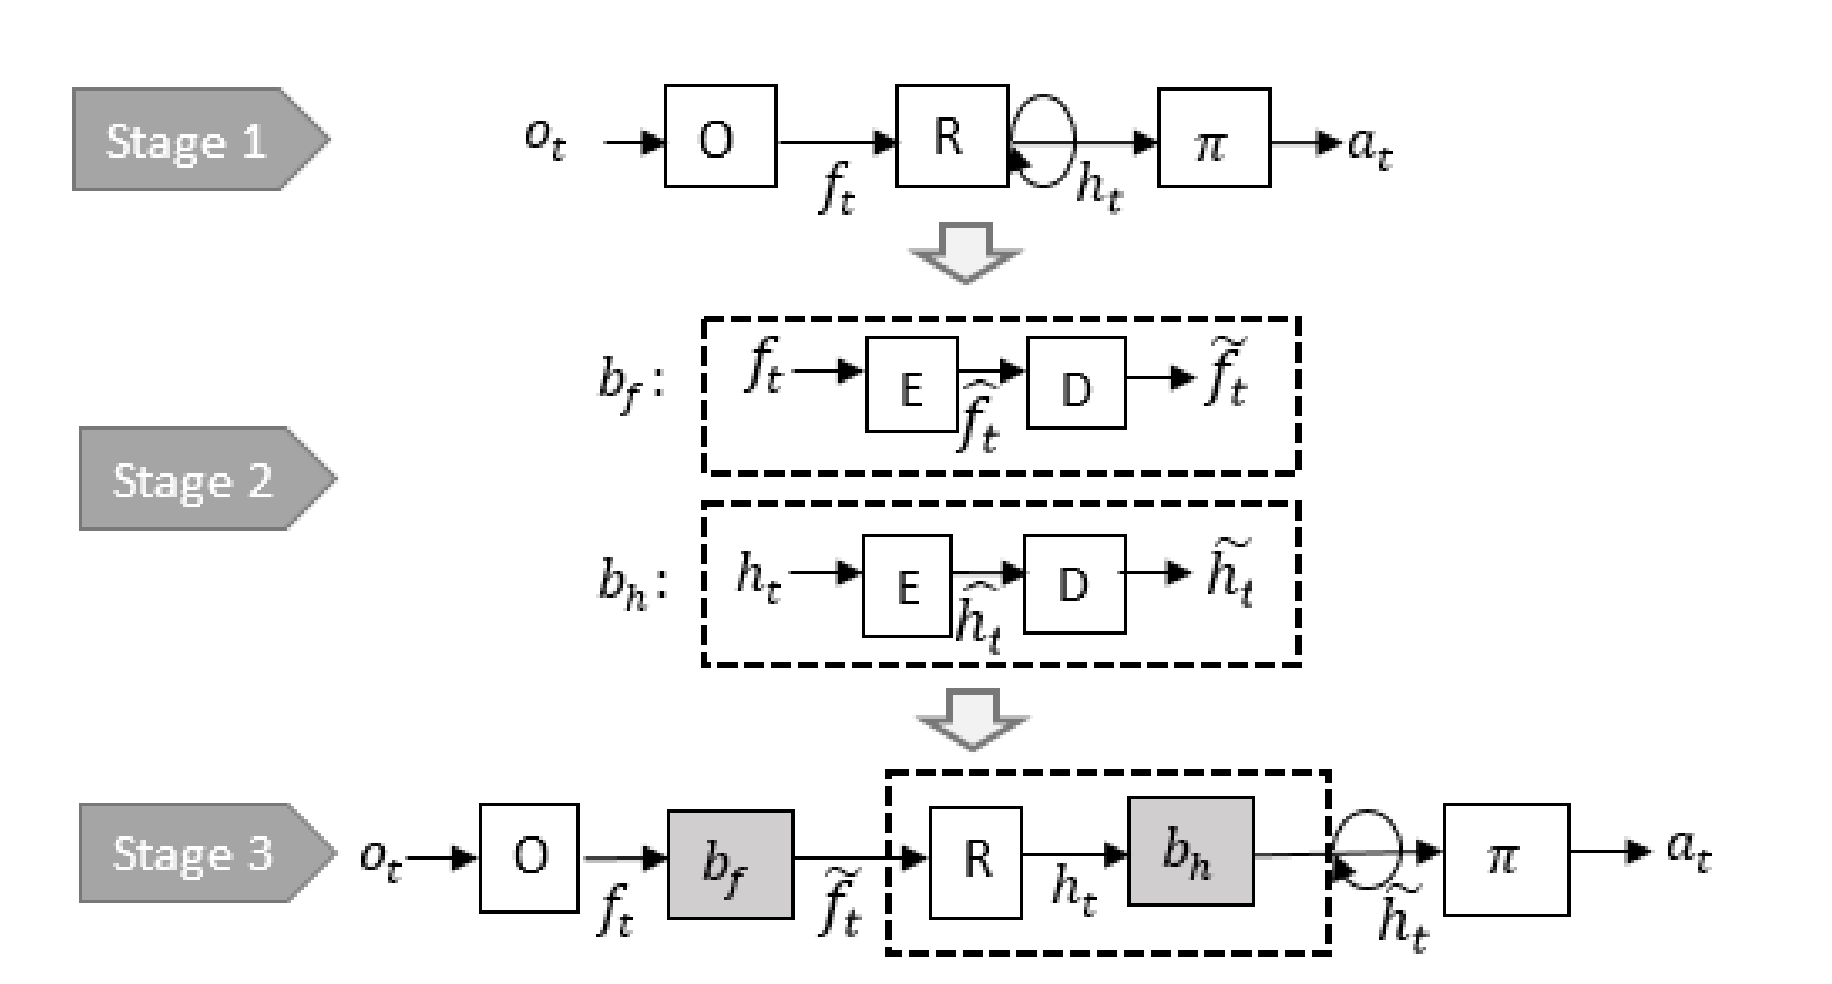
\includegraphics[width=\textwidth]{Figures/net_architecture_overview.png}
    \caption{The conceptual building steps for the moore machine network \cite{Koul2019}. Note that the bottlenecks ($b_f$ and $b_h$) are trained separately and \textit{then} inserted in the regular policy ($o_t-O-R-h_t-\pi-a_t$).}
    \label{fig: net_architecture_overview}
\end{figure}


Here is a high-level overview of the steps I took to learn a
moore machine network (MMN) controller, following Koul et. al. \cite{Koul2019}, with the high-level steps for the process shown in Figure \ref{fig: net_architecture_overview}:

\begin{enumerate}
\def\labelenumi{\arabic{enumi}.}
\item
  Learn an feature\_extractor-rnn\_policy for a RL environment using a
  standard RL algorithm capable of learning with a recurrent policy,
  \href{https://openai.com/blog/openai-baselines-ppo/}{PPO2}. PPO is a policy gradient method that essentially allows for monotonic policy improvements like in TRPO \cite{TRPO}\cite{PPO2}. It develops a "surrogate" objective function $L_{t}^{C L I P+V F+S}(\theta)$ that can be approximately mazimized each step \cite{PPO2}:
  
  \(L_{t}^{C L I P+V F+S}(\theta)=\hat{\mathbb{E}}_{t}\left[L_{t}^{C L I P}(\theta)-c_{1} L_{t}^{V F}(\theta)+c_{2} S\left[\pi_{\theta}\right]\left(s_{t}\right)\right]\)
  
  Where $L_{t}^{C L I P}(\theta)$ is the clipped surrogate objective that is the basis for the whole procedure, where it lower bounds another constrained policy objective, the conservative policy iteration objective \cite{PPO2}. $c_{1} L_{t}^{V F}(\theta)$ is the scaled value estimate produced by the actor-critic portion of the policy network, and $S\left[\pi_{\theta}\right]\left(s_{t}\right)$ is an entropy bonus to encourage the production of explorative actions (we don't want too simple of a policy - likely not a good one) \cite{PPO2}.
  
  Here the feature extraction network is known as \texttt{F\_ExtractNet} and the
  RNN policy that takes these features and produces the next action is
  known as \texttt{RNN\_Policy}. \emph{If your environment already has
  simple, discrete observations, you will not need
  \texttt{F\_ExtractNet} and can directly feed the observation into the
  \texttt{RNN\_Policy}.} Here, we use the \href{https://stable-baselines.readthedocs.io/}{stable-baselines} implementation of PPO2 with our custom policy networks to train the CNN-LSTM agent \cite{stable-baselines}.
\item
  Generate ``Bottleneck Data''. This is where you simulate many
  trajectories in the RL environment, recording the observations and the
  actions taken by the \texttt{RNN\_Policy}. This is for training the
  ``quantized bottleneck neural networks'' (\texttt{QBNs}) next.
\item
  Learn \texttt{QBNs}, which are essentially applied autoencoders (AE),
  to quantize (discretize):

  \begin{itemize}
  \itemsep1pt\parskip0pt\parsep0pt
  \item
    the observations of the environmental feature extractor:

    \begin{itemize}
    \itemsep1pt\parskip0pt\parsep0pt
    \item
      CNN if using an agent that observes video of the environment.
    \item
      MLP if getting non-image state observations This is called
      \texttt{b\_f} in the paper and \texttt{OX} in the mnn code.
    \end{itemize}
  \item
    the hidden state of the \texttt{RNN\_Policy}. This is called
    \texttt{b\_h} in the paper and \texttt{BHX} in the mnn code
  \end{itemize}
\end{enumerate}

    This is done by taking the bottleneck data and using to train the QBNs as if they were autoencoders, using a reconstructive MSE loss on the input and reconstructed input from the QBN. One thing worth noting here is that in order for the QBN's quantized state comes from using a ternary activation on the inputs to the latent layer \cite{Koul2019}. This way, each hidden neuron in the latent layer of each QBN has a value of either -1, 0, or 1. In this way, we gain a compressed AND quantized representation of the input at the latent layer of the network.

    This ternary activation $\phi$ is given by \(\phi(x)=1.5 \tanh (x)+0.5 \tanh (-3 x)\) \cite{Koul2019}. As suggested by Koul et. al., we must find a way to estimate the gradient of this activation, as it is non-differentiable. Koul et. al., referencing work by others in quantization of network representations, treats the function as the identity during backprop \cite{Koul2019}.

\begin{enumerate}
\def\labelenumi{\arabic{enumi}.}
\setcounter{enumi}{3}
\item
  Inserting the trained \texttt{OX} QBN \emph{before} the feature extractor
  and the trained \texttt{BHX} QBN \emph{after} the RNN unit in the
  feature\_extractor-rnn\_policy network to create what is now called
  the moore machine network (\texttt{MMN}) policy.
\item
  Fine-tune the \texttt{MMN} policy by re-running the rl algorithm using
  the \texttt{MMN} policy as a starting point for RL interactions.
  \emph{Importantly, for training stability the \texttt{MMN} is
  fine-tuned to match the softmax action distribution of the original
  \texttt{RNN\_Policy}, not the argmax -\textgreater{} optimize with a
  categorical cross-entropy loss between the RNN and \texttt{MMN} output
  softmax layers}.
\end{enumerate}


\begin{table}[H]
\caption{Network Architecture for the CNN-LSTM Policy Trained with PPO2. Input flows sequentially downwards through layers unless otherwise noted.}
\label{t: ppo2_arch}
\begin{tabular}{a b}
      \toprule
      \thead{\textbf{Layer Name}} & \thead{\textbf{Layer Parameters}} \\
      \midrule
      conv1                & n\_filt=32, filt\_size=8, stride=4, bias=True, act=ReLU \\
      conv1                & n\_filt=32, filt\_size=8, stride=4, bias=True, act=ReLU \\
      conv1                & n\_filt=32, filt\_size=8, stride=4, bias=True, act=ReLU \\
      fc1                  & n\_hidden=512, bias=True, act=ReLU \\
      LSTM                 & n\_hidden\_cells=256, act=Tanh\\
      value\_est\_fc       & n\_hidden=1, act=Linear (linked to LSTM out)\\
      actions\_dist\_fc    & n\_hidden=n\_actions=6, act=softmax (linked to LSTM out)\\
      Q\_est\_fc           & n\_hidden=n\_actions=6, act=Linear (linked to LSTM out)\\
      \bottomrule
\end{tabular}
\centering
\end{table}

\begin{table}[H]
\caption{Hyperparameters for the CNN-LSTM Policy Trained with PPO2}
\label{t: ppo2_hparams}
\begin{tabular}{a b}
      \toprule
      \thead{\textbf{Hyperparameter Name}} & \thead{\textbf{Value}} \\
      \midrule
       n\_parallel\_envs & 16 \\
       cliprange & linear\_decay(0.1)\\
       ent\_coef & 0.01\\
       $\gamma$ & 0.99\\
       $\lambda$ & 0.95\\
       learning rate & linear\_decay(4e-4)\\
       optimizer & Adam() default betas \\
       n\_steps & 128\\
       n\_timesteps & 7,000,000\\
       nminibatches & 8\\
       noptepochs & 4\\
      \bottomrule
\end{tabular}
\centering
\end{table}

\begin{table}[H]
\caption{Network Architecture for the Observation Feature QBN. Input flows sequentially downwards through layers unless otherwise noted.}
\label{t: obs_qbn_arch}
\begin{tabular}{a b}
      \toprule
      \thead{\textbf{Layer Name}} & \thead{\textbf{Layer Parameters}} \\
      \midrule
      fc1-enc              & n\_hidden=fc3\_out.flatten()=512, act=Tanh\\
      fc2-enc              & n\_hidden=8*n\_latent\_states=800, act=Tanh\\
      latent-enc           & n\_hidden=100, act=ternary\_tanh\\
      fc1-dec              & n\_hidden=8*n\_latent\_states=800, act=Tanh\\
      fc2-dec              & n\_hidden=512, act=ReLU6\\
      \bottomrule
\end{tabular}
\centering
\end{table}

\begin{table}[H]
\caption{Hyperparameters for the Observation Feature QBN}
\label{t: obs_qbn_hparams}
\begin{tabular}{a b}
      \toprule
      \thead{\textbf{Hyperparameter Name}} & \thead{\textbf{Value}} \\
      \midrule
       learning rate & linear\_decay(4e-4)\\
       optimizer & Adam() default betas \\
       \thead{global norm \\ gradient clip} & \thead{5.0}\\
       loss & MSE\\
       batch\_size & 32\\
       epochs & 600\\
       n\_training\_ex & 5000\\
      \bottomrule
\end{tabular}
\centering
\end{table}

\begin{table}[H]
\caption{Network Architecture for the Hidden State Feature QBN. Input flows sequentially downwards through layers unless otherwise noted.}
\label{t: hid_state_qbn_arch}
\begin{tabular}{a b}
      \toprule
      \thead{\textbf{Layer Name}} & \thead{\textbf{Layer Parameters}} \\
      \midrule
      fc1-enc              & n\_hidden=fc3\_out.flatten()=256, act=Tanh\\
      fc2-enc              & n\_hidden=8*n\_latent\_states=640, act=Tanh\\
      fc3-enc              & n\_hidden=4*n\_latent\_states=320, act=Tanh\\
      latent-enc           & n\_hidden=80, act=ternary\_tanh\\
      fc1-dec              & n\_hidden=4*n\_latent\_states=320, act=Tanh\\
      fc2-dec              & n\_hidden=8*n\_latent\_states=640, act=Tanh\\
      fc3-dec              & n\_hidden=512, act=Tanh\\
      \bottomrule
\end{tabular}
\centering
\end{table}

\begin{table}[H]
\caption{Hyperparameters for the Hidden State Feature QBN}
\label{t: hid_state_qbn_hparams}
\begin{tabular}{a b}
      \toprule
      \thead{\textbf{Hyperparameter Name}} & \thead{\textbf{Value}} \\
      \midrule
       learning rate & linear\_decay(4e-4)\\
       optimizer & Adam() default betas \\
       \thead{global norm \\ gradient clip} & 5.0\\
       loss & MSE\\
       batch\_size & 32\\
       epochs & 600\\
       n\_training\_ex & 5000\\
      \bottomrule
\end{tabular}
\centering
\end{table}